\label{Konzept}
\chapter{Konzept}

\section{Grundkonzept}

\begin{figure} %[hbtp]
   \centering
   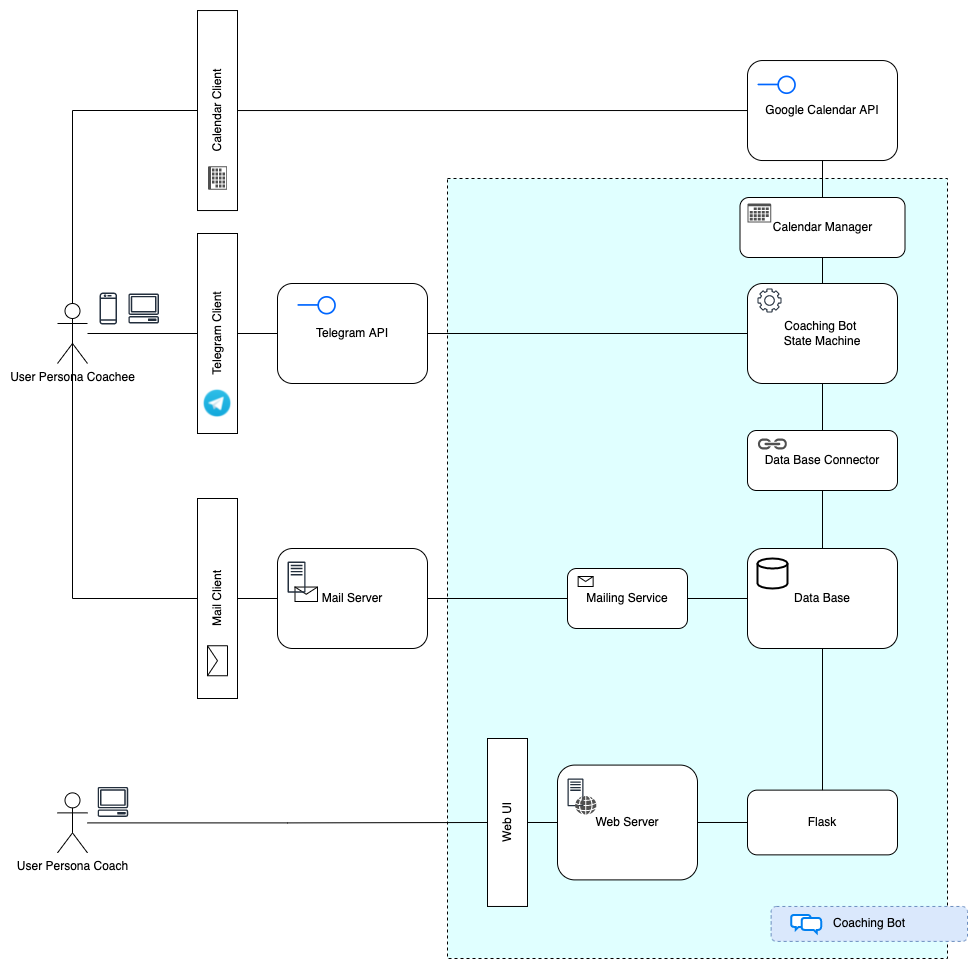
\includegraphics[width=1.0\textwidth]{images/220320_PA28464_Architecture.png}
   \caption{Konzeptionelle Architektur für das Projekt \emph{Der Coaching Bot}}
   \label{fig: Abbildung 1 - Konzeptionelle Architektur für das Projekt "Der Coaching Bot"}
\end{figure}

Der Kern des Bots basiert auf einem endlichen Automaten (state machine), der Zustände vordefiniert und festlegt, wann sich welcher Nutzer in welchem Zustand befindet und von welchem in welchen Zustand er sich bewegen darf. An diesen Kern bindet sind als zentrales Steuerungselement des Bots alle anderen Systeme angebunden. Dazu gehören:
\begin{enumerate}
	\item Die Datenbank zur Speicherung der Nutzerdaten
	\item Die Telegram API, über die die Kommunikation mit dem Telegram Client abgewickelt wird
	\item Die Google Calendar API, über die Events erstellt und versendet werden können
	\item Den Mail Server, über den E-Mails an den nutzer versendet werden können.
\end{enumerate} 

Der Nutzer interagiert mit dem ganzen System durch vier Kanäle:
\begin{enumerate}
	\item Telegram Client: Kommunikation mit dem Bot
	\item Calendar Client: Erhalt, Annahme sowie Ablehnung der vereinbarten Termine
	\item Mail Client: Erhalten der Zusammenfassung und Bestätigung
	\item Web Browser: Übersicht über Anmeldungen und Terminkalender
\end{enumerate}

Der Bot wird von Benutzern via einem Telegram Client angesprochen und reagiert auf die Eingabe entsprechend. So können verschieden Funktionen ausgelöst werden. Bspw. werden Antworten zurückgegeben, Informationen gespeichert oder es wird ein Vorschlag gemacht und an den Nutzer zurückgegeben. Der Bot soll mit mehreren Benutzern gleichzeitig sprechen können. Das wird ermöglicht, weil alle Reaktionen des Bots mit der Kennung des jeweiligen Nutzers verknüpft sind. So spricht der Bot den Nutzer mit Namen an oder kann sich daran erinnnern, welche Fragen schon beantwortet wurden und welche nicht. \\ \\

Daneben gibt es einen zweite, sehr einfache Web-Applikation, die auf Flask basiert und eine Web-GUI zur Verfügung stellt, über die die gesammelten Informationen dargestellt werden können. So kann ein Coach sich, nachdem Bewerber den Prozess beendet haben, alle gesammelten Informationen sowie vereinbarte Termine in einer einfachen Web-GUI ansehen.


\begin{figure} %[hbtp]
	\centering
	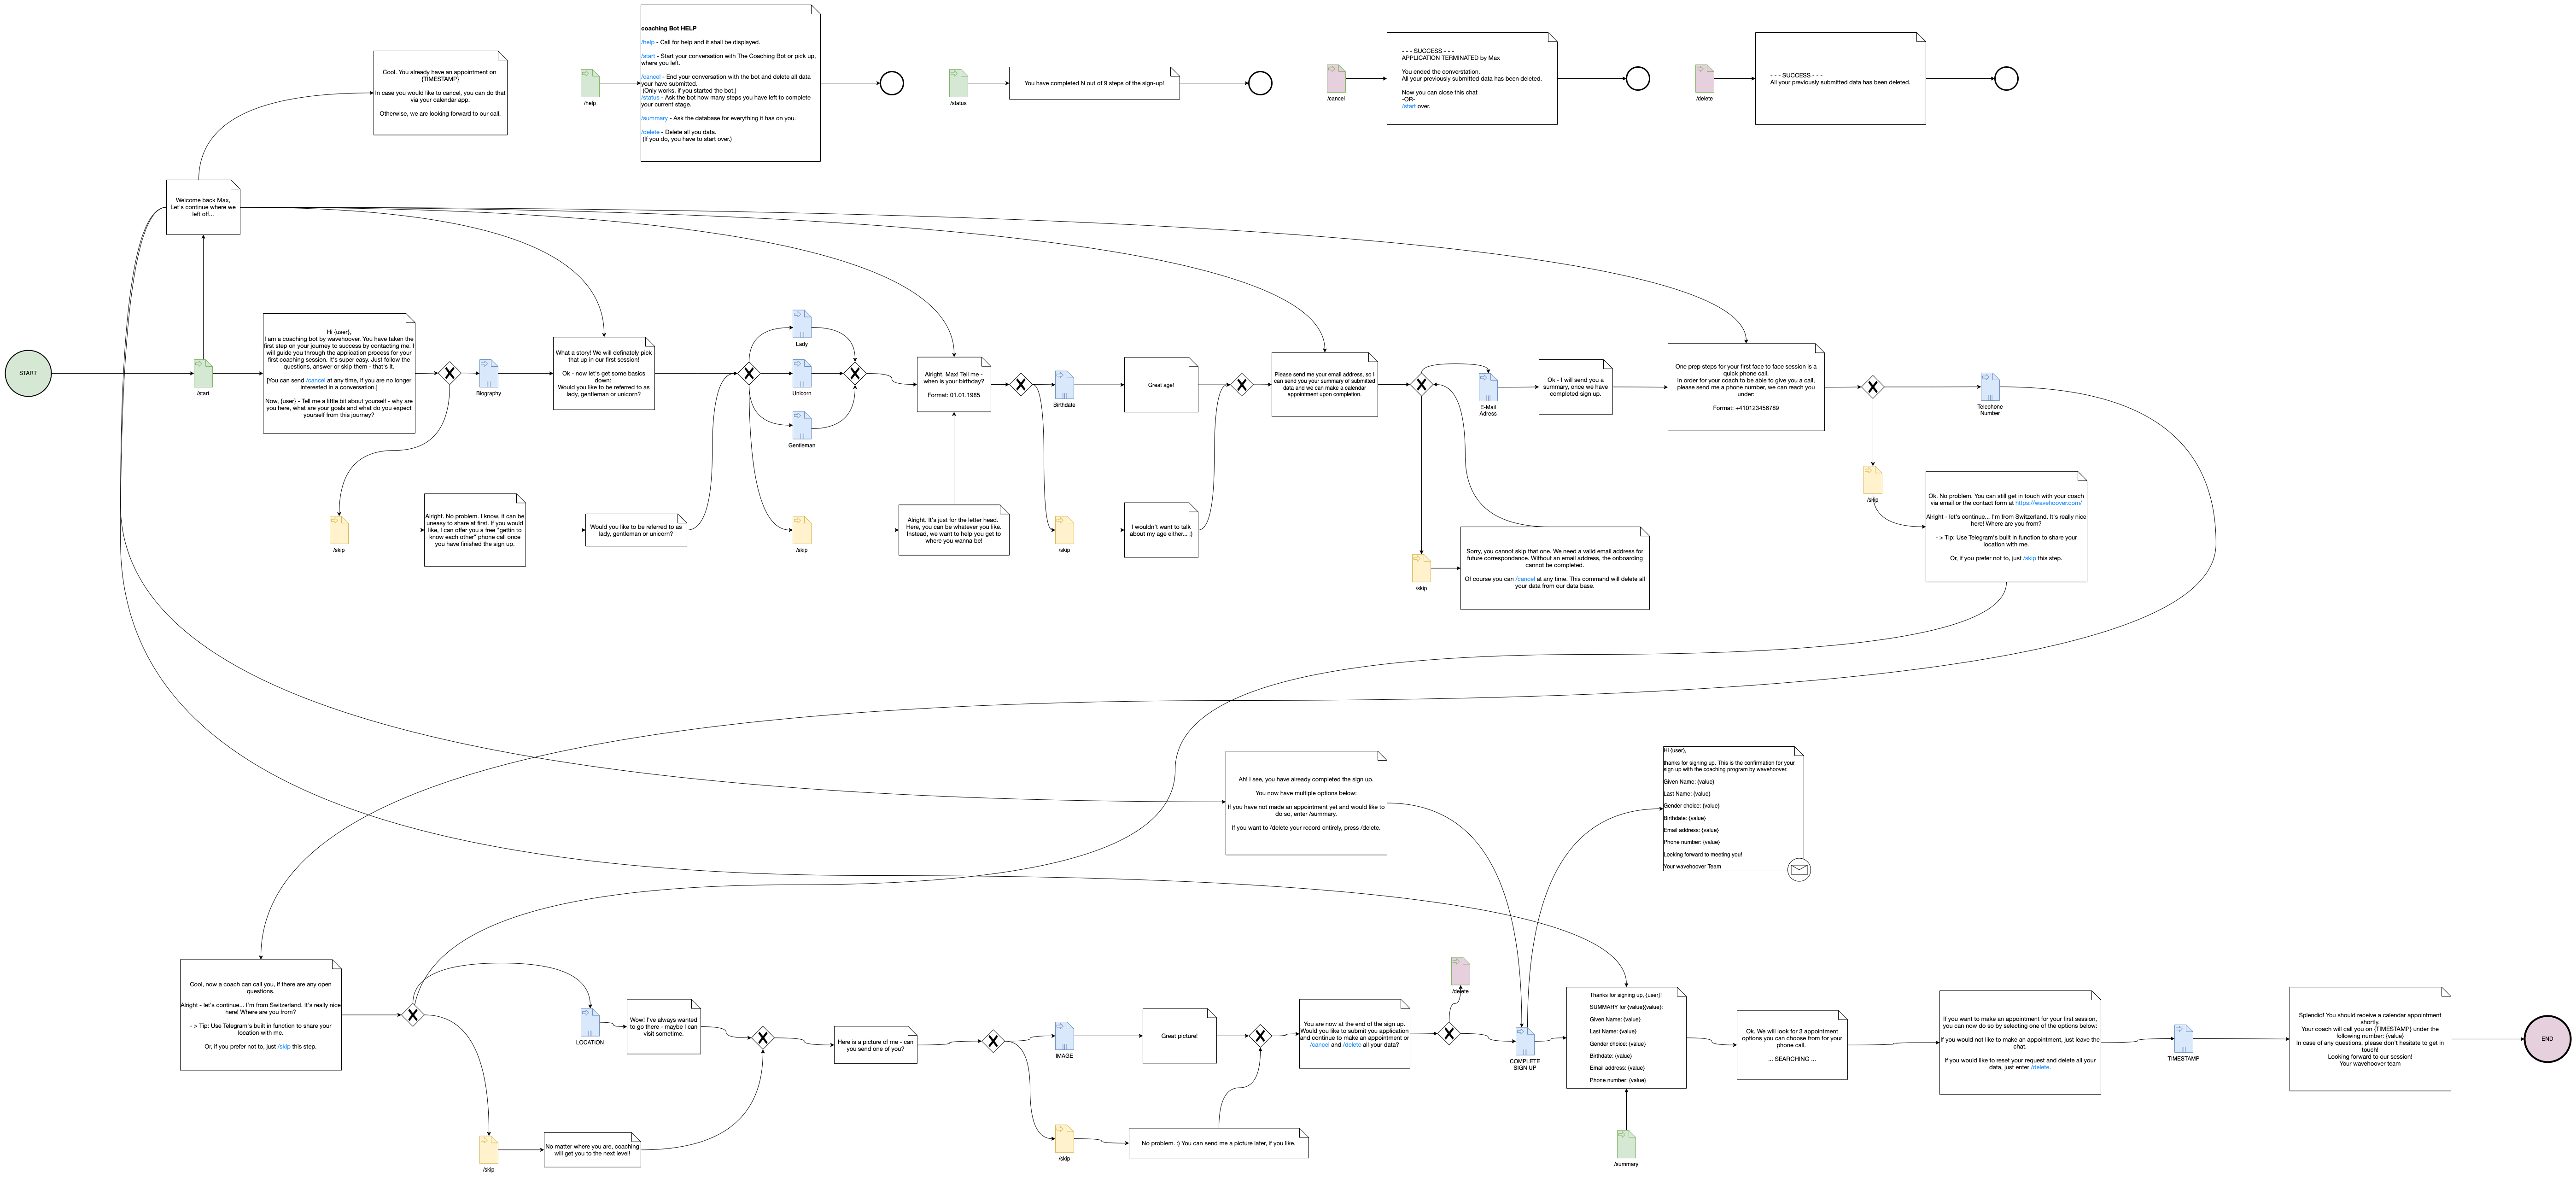
\includegraphics[width=1.0\textwidth]{images/220213_PA28464_Conversation_Flow.png}
	\caption{Konversationsfluss des Bots}
	\label{conversationFlow}
\end{figure}

